The Widget Manager serves as the portal through which developers can contribute their widgets to the community by uploading them to the store. To streamline the onboarding process, account creation and widget submission are facilitated by a simple "Sign in with GitHub" option, requiring only a single tap to initiate. This reduces friction and ensures ease of access for new contributors.

Upon signing in, developers gain immediate access to their dashboard, where they can view a list of previously developed widgets, create new ones, or modify existing submissions.

\begin{figure}[h] \centering \begin{minipage}[b]{0.49\textwidth} \centering 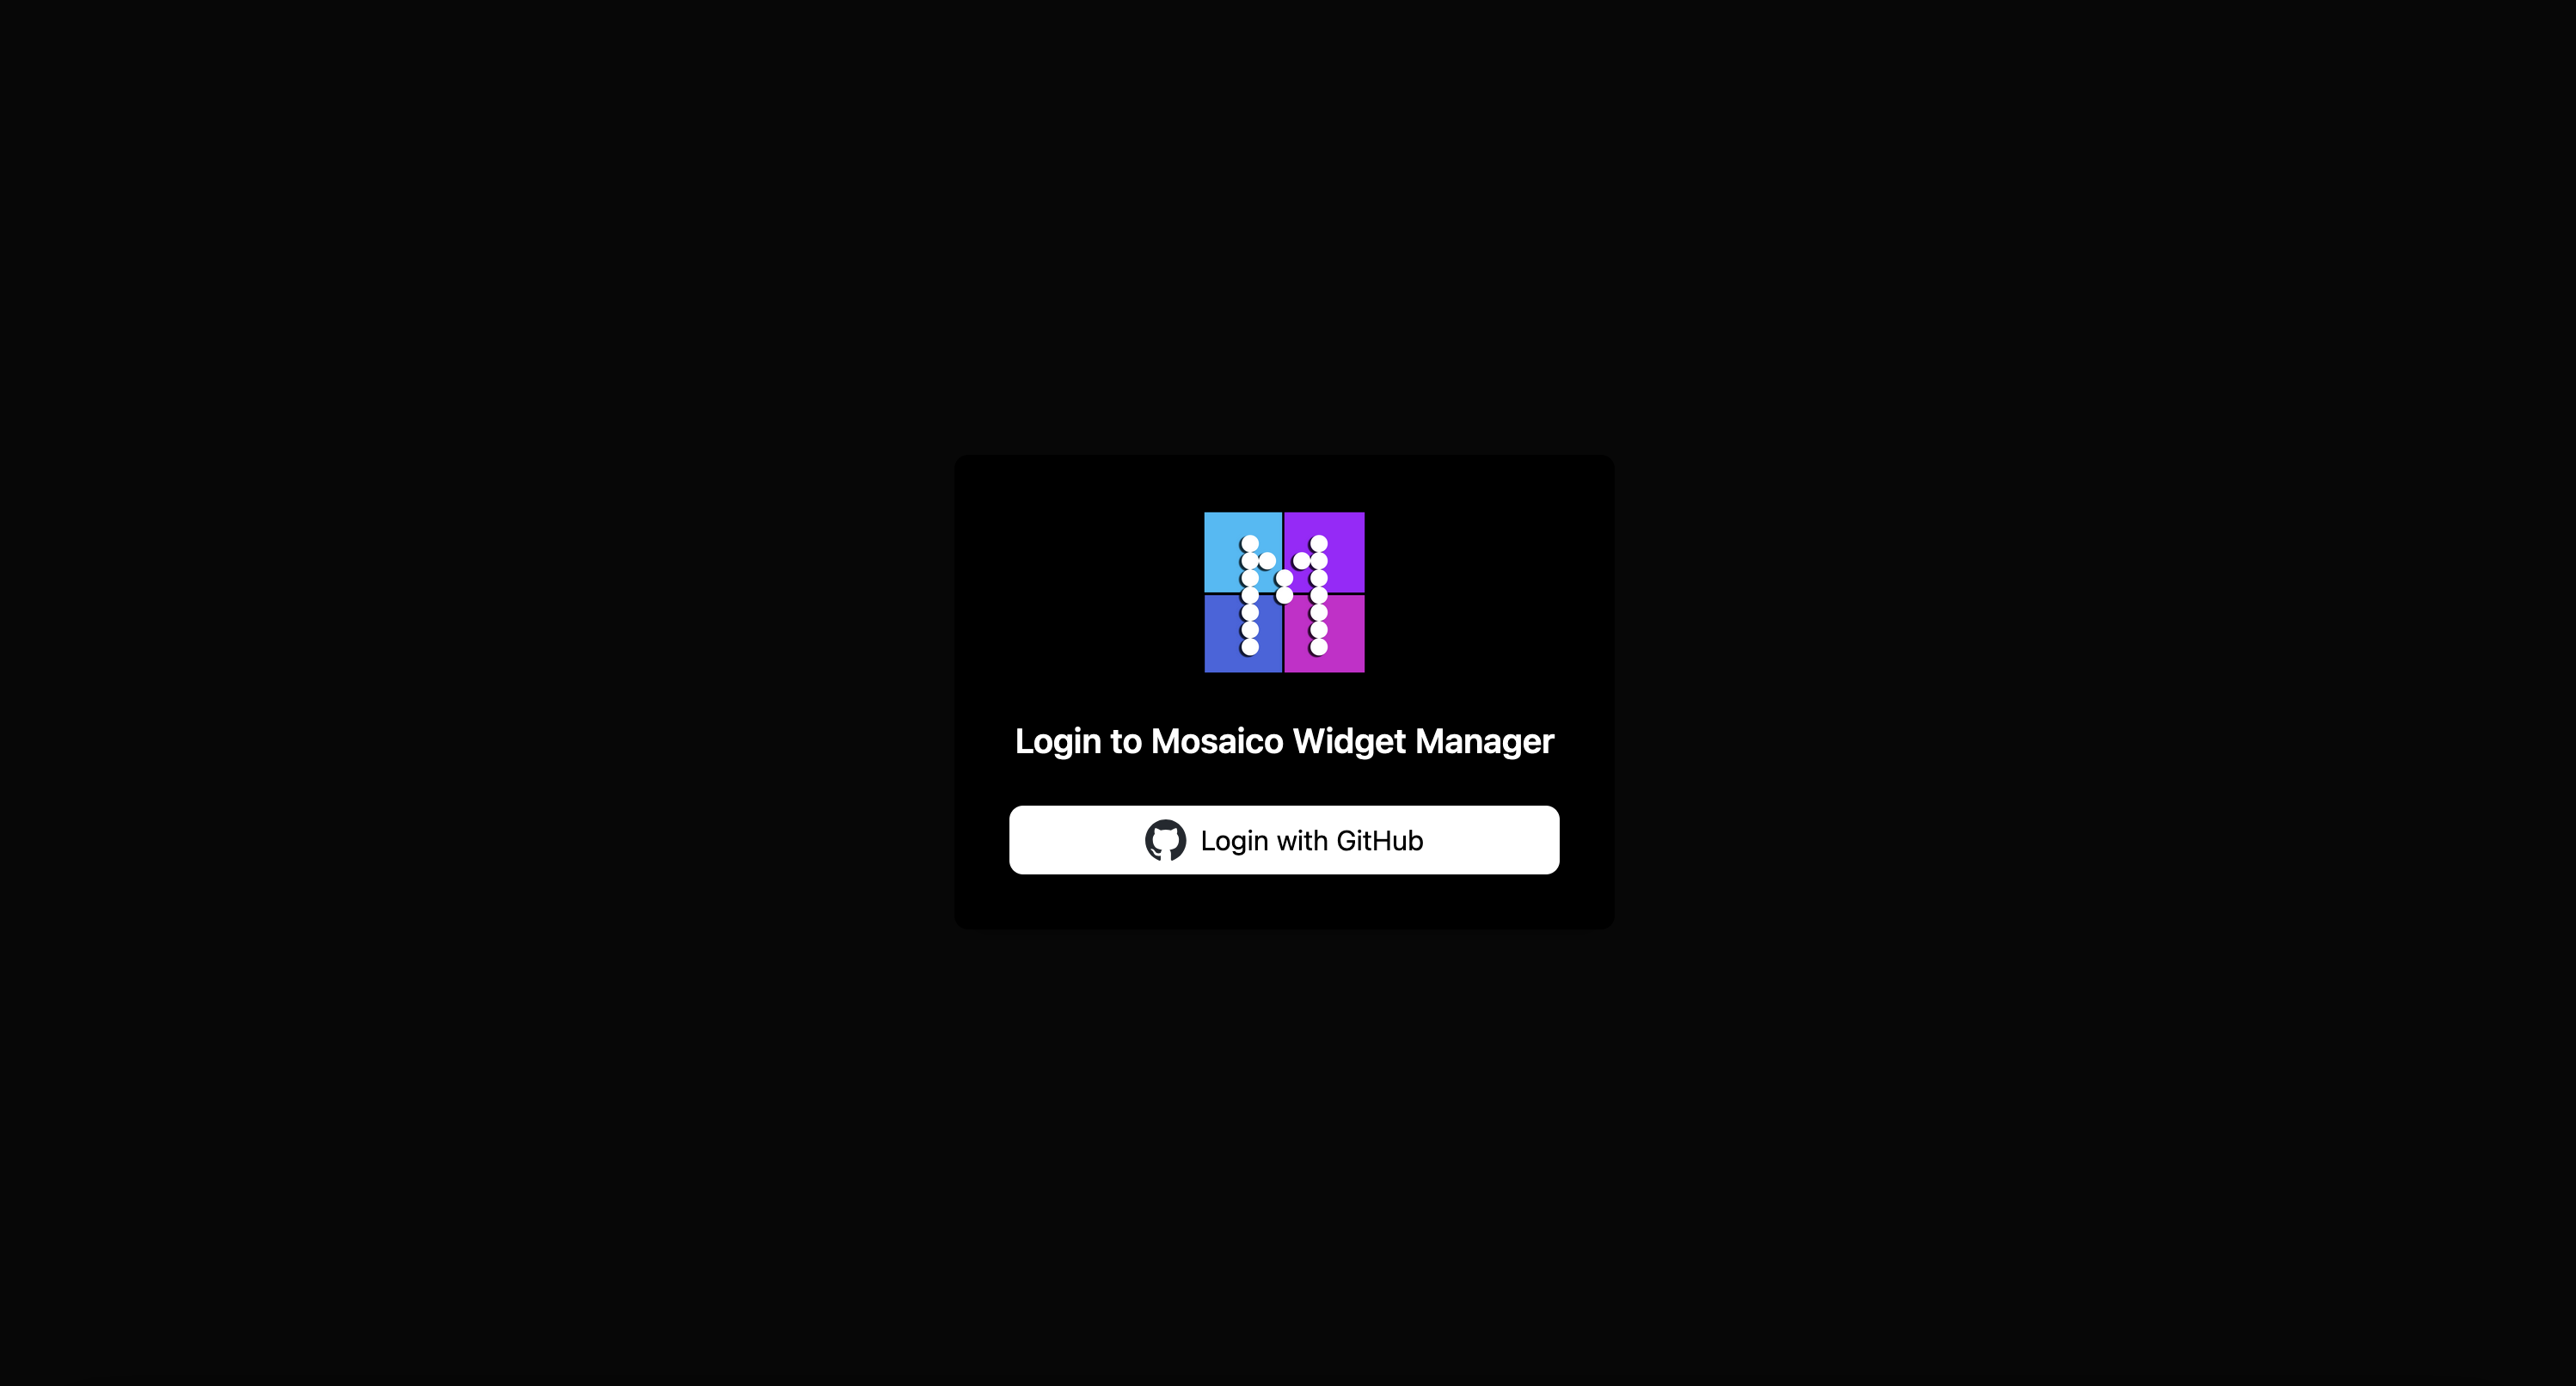
\includegraphics[width=\textwidth]{tesi/img/website_demo/login.png} \caption*{Login with GitHub} \end{minipage} \begin{minipage}[b]{0.49\textwidth} \centering 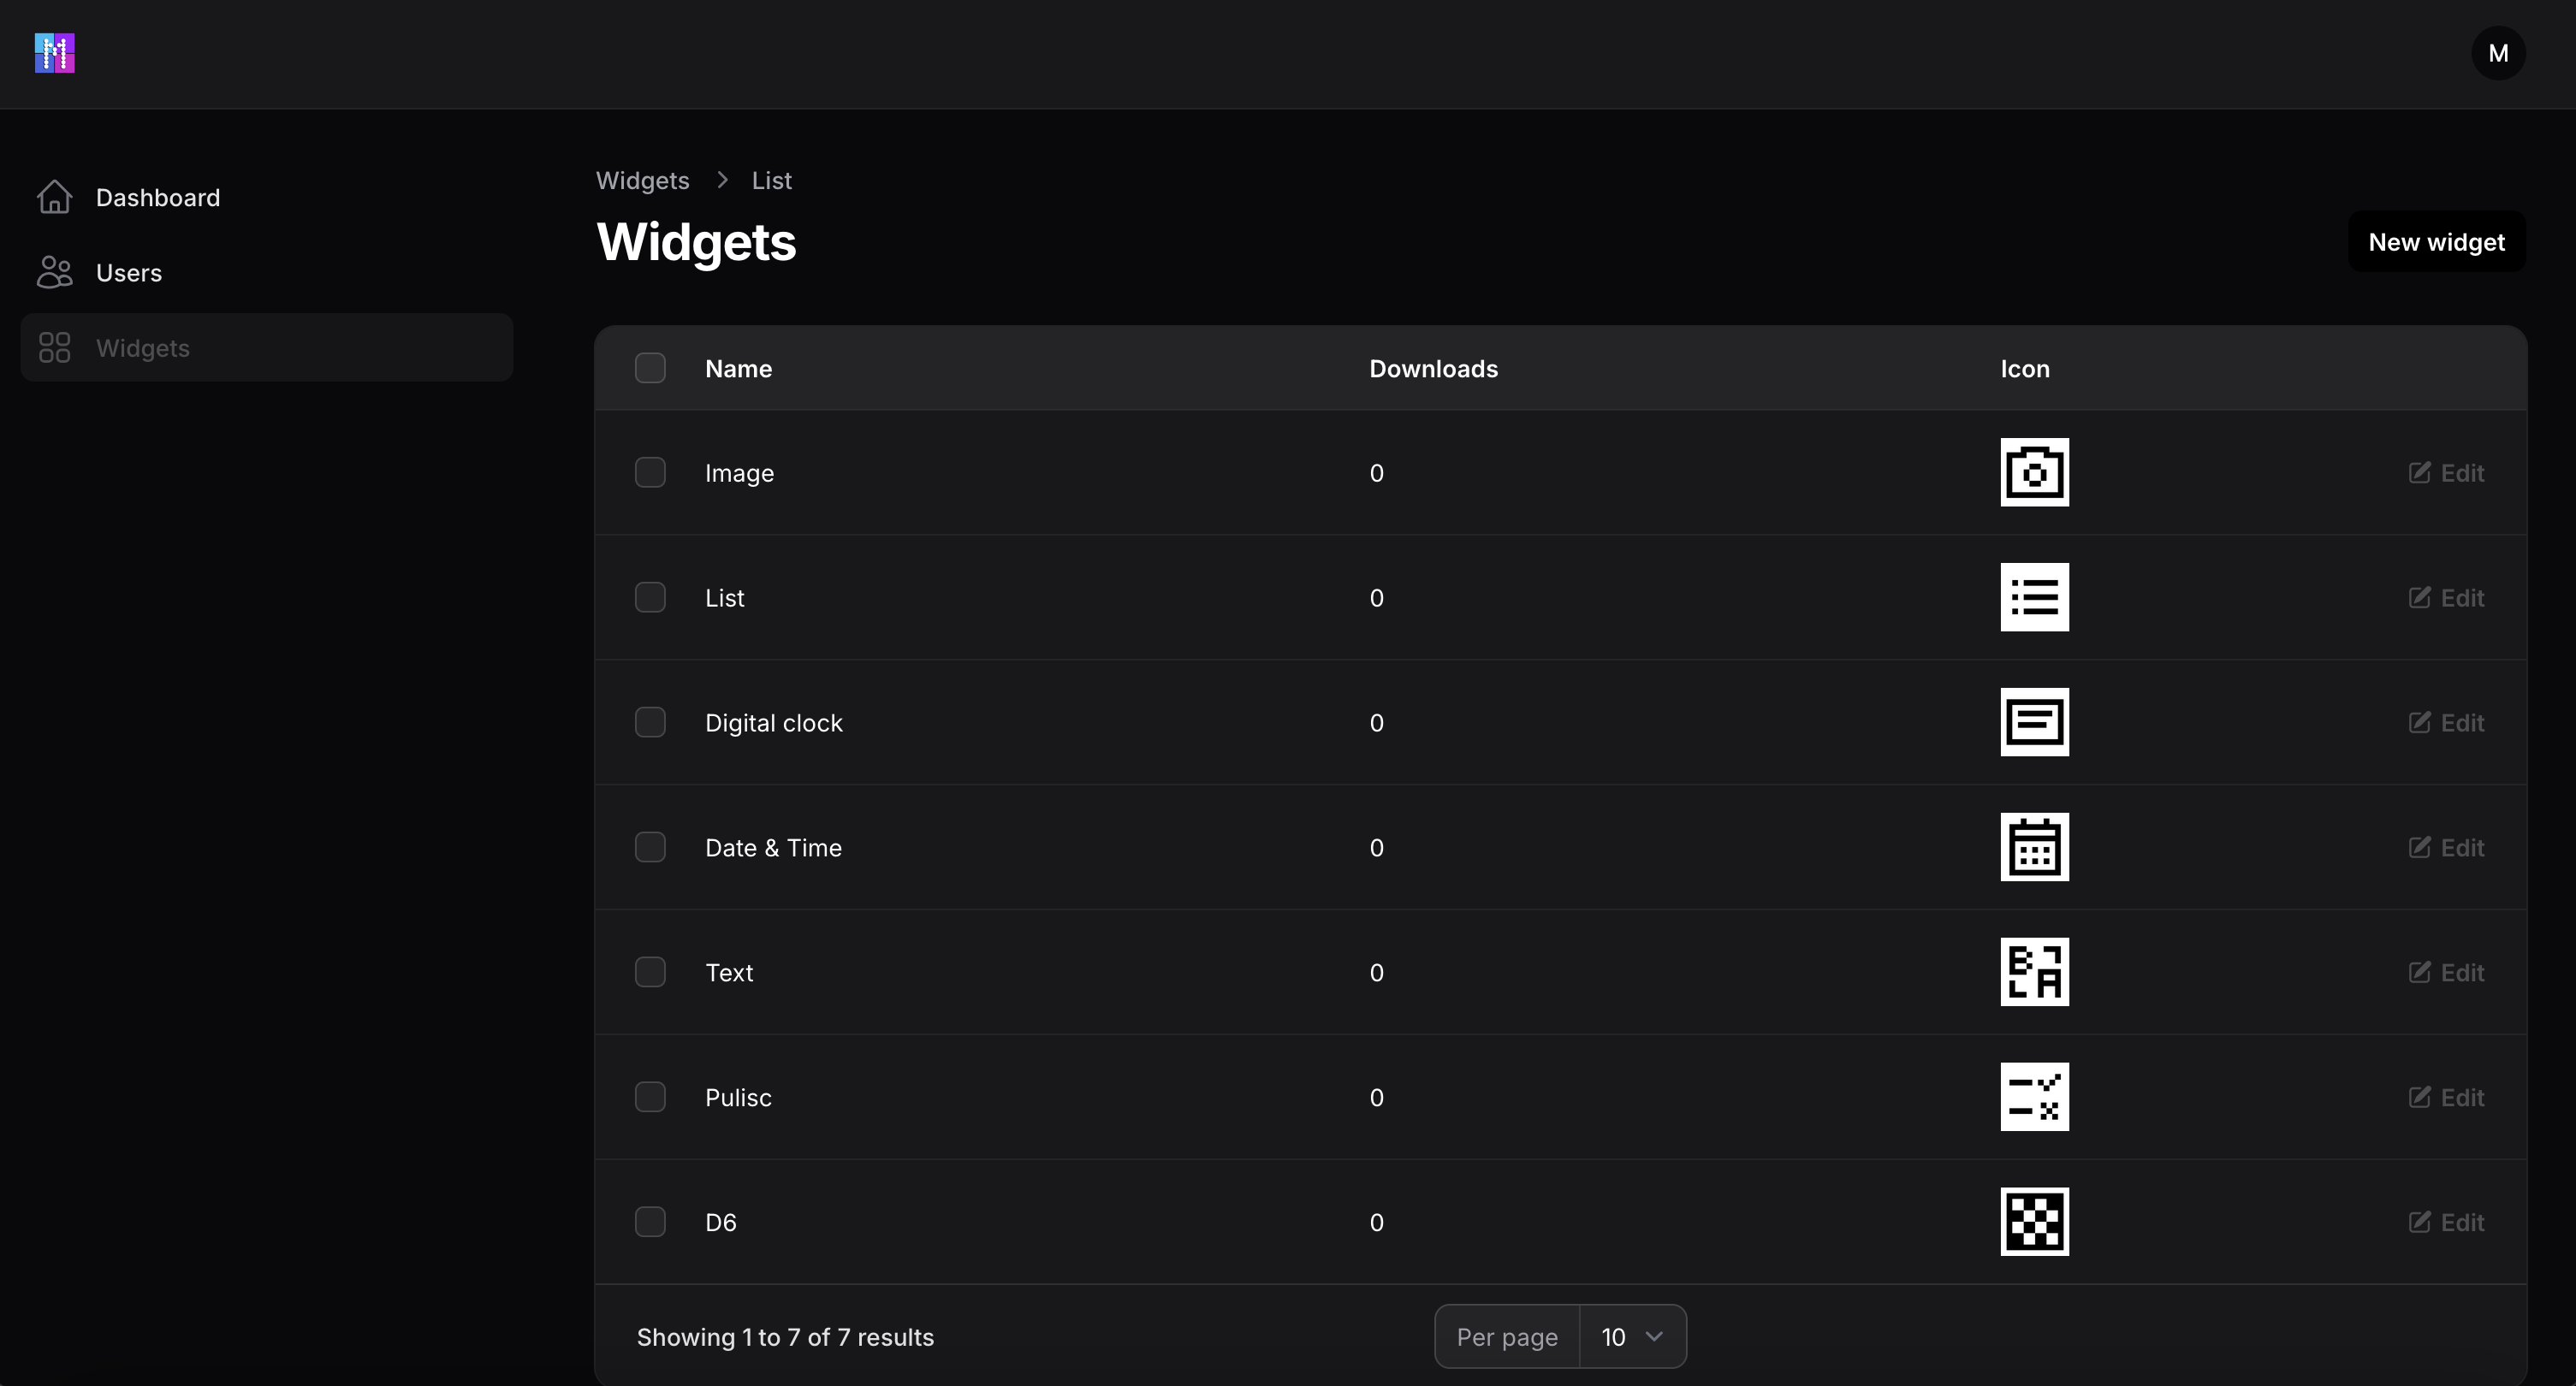
\includegraphics[width=\textwidth]{tesi/img/website_demo/widgets.png} \caption*{Developer's Widgets} \end{minipage} \end{figure}

The user interface has been designed to be intuitive and accessible, ensuring that developers can easily manage their contributions. Developers are required to provide the following information for each widget submission:

\begin{itemize} \item Name of the widget \item An icon representing the widget \item A short tagline or description, displayed beneath the widget’s name \item A comprehensive markdown description, which will appear on the store page \item A series of images, presented in a carousel on the store page \item A link to a valid Git repository, from which the widget can be downloaded \end{itemize}

\begin{figure}[h] \centering \begin{minipage}[b]{0.49\textwidth} \centering 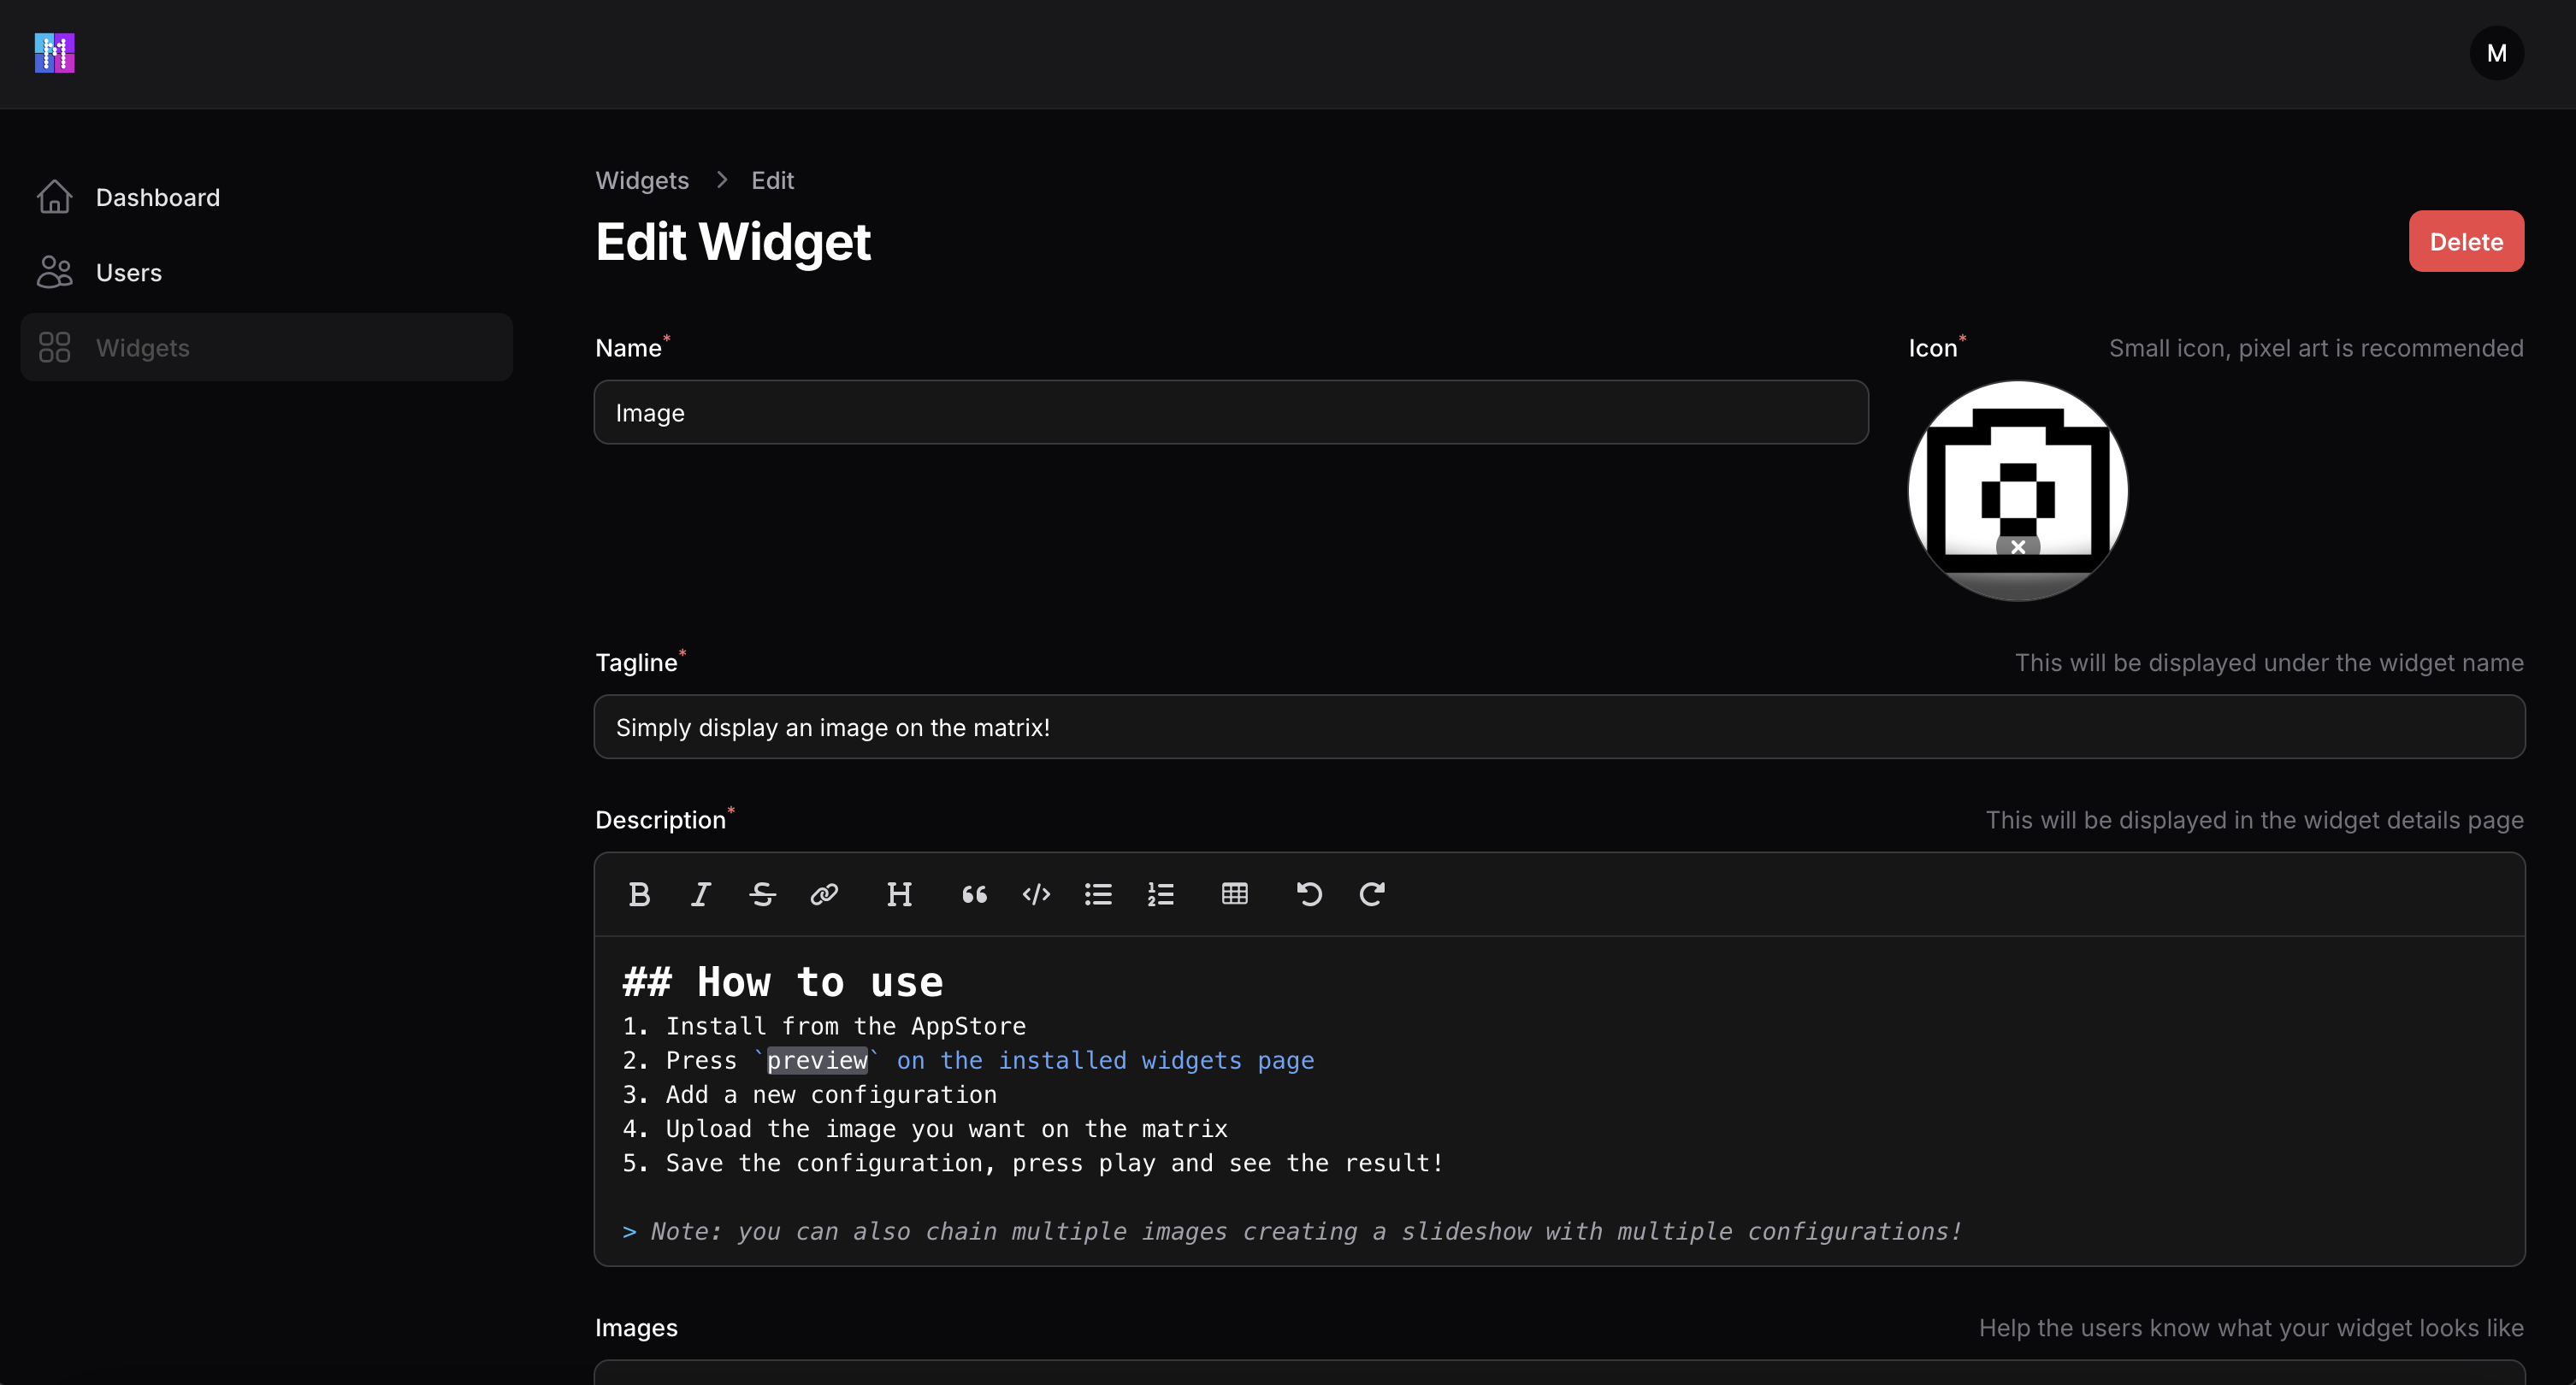
\includegraphics[width=\textwidth]{tesi/img/website_demo/widget-details.png} \caption*{Edit Widget} \end{minipage} \begin{minipage}[b]{0.49\textwidth} \centering 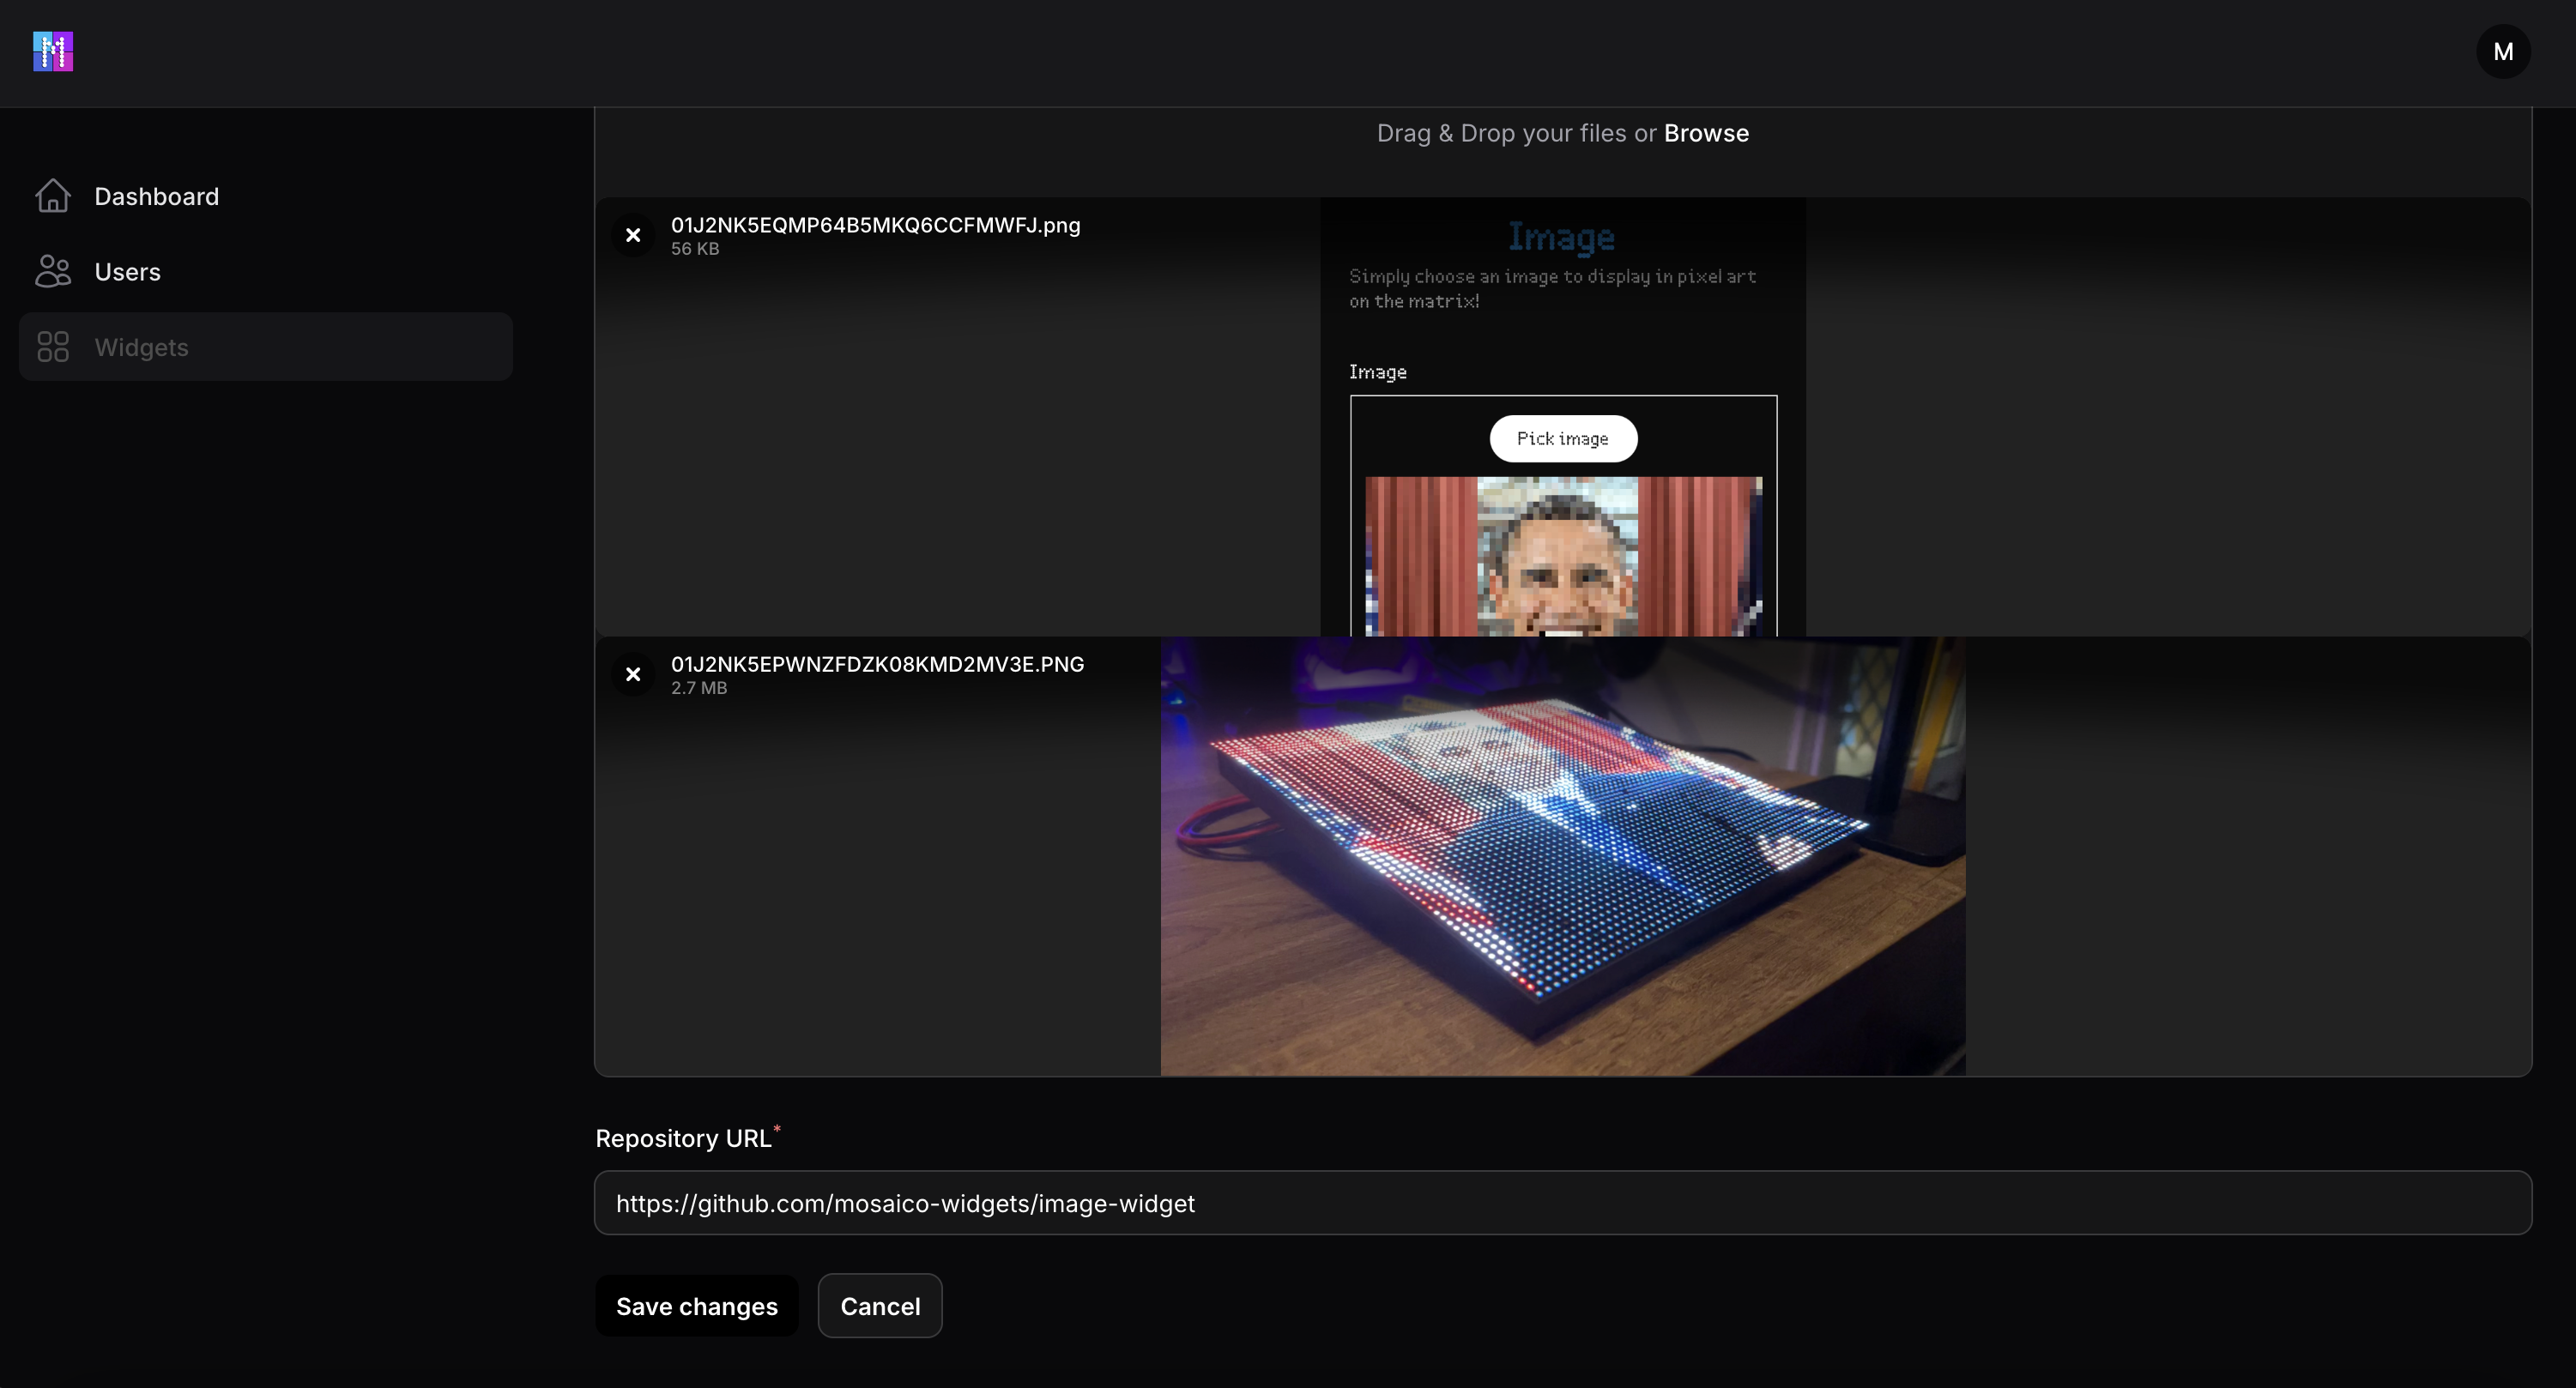
\includegraphics[width=\textwidth]{tesi/img/website_demo/widget-details-2.png} \caption*{Edit Widget - Continued} \end{minipage} \end{figure}

Once all necessary fields have been completed and the developer saves their submission, the widget becomes immediately available to the community.